%%Präambel--------------------------------------------------

%Dokument erstellen
\documentclass
[a4paper,
 DIV11,
 bibliography=totoc,
 headings=normal,
 ngerman,
 headsepline,
 listof=totoc,
 parskip=half
]{scrreprt}

%Packages laden
%Benötigte Packages
\usepackage{babel} 
\usepackage[T1]{fontenc}           
\usepackage[utf8]{inputenc}  
\usepackage{graphicx}
\usepackage{amsmath}
\usepackage{lmodern}
\usepackage[printonlyused,withpage]{acronym}
\usepackage[a4paper,margin=2cm]{geometry}
\usepackage{amssymb} 
\usepackage{amsmath,amsthm}
\usepackage{textcomp}
\usepackage{setspace}
\usepackage{scrpage2}
\usepackage{blindtext}
\usepackage{graphicx}
\usepackage{amsthm}
\usepackage{blindtext}
\usepackage[pdfborder={0 0 0}]{hyperref}
\usepackage{mdframed}
\usepackage{float}
\usepackage{subfigure}
\usepackage{listings}
\usepackage{booktabs}

\usepackage{helvet}
\renewcommand{\familydefault}{\sfdefault}
\newcommand{\tabitem}{~~\llap{\textbullet}~~}
\fontfamily{phv}\selectfont

\usepackage
[activate={true,nocompatibility}, %activate protrusion and expansion
 final,							  %final: enable microtype draft:disable
 tracking=true,                   %activate tracking  
 kerning=true,					  %activate kerning
 spacing=true,                    %activate spacing
 factor=1100,					  %add 10% to the protrusion (default is 1000)
 stretch=10,					  %reduce stretchability (default is 20)
 shrink=10						  %reduce shrinkability (default is 20)
]{microtype}

              


%PDFInfos laden
%Informationen der PDF
\pdfinfo
{
/Title		(Extrapolation von Zeitreihen mit Hilfe von künstlichen neuronalen Netzen am Beispiel von Börsenprognosen)
/Subject	(Eine Anwendung im Fach Softcomputing – Teilgebiet neuronale Netze)
/Author		(Sebastian Schötteler \& Benedikt Hofrichter)
}


%Seitenstil laden
%Zeilenabstand 1,5
\onehalfspacing

%Kopfzeilen, Fußzeilen und Seitennummerierung setzen
\pagestyle{scrheadings}
\clearscrheadfoot
\automark{chapter}
\ohead[]{\headmark} % Kapitel
\ofoot[\pagemark]{\pagemark} %Seitenzahl
\ifoot{Sebastian Schötteler \& Benedikt Hofrichter} %Verfasseer

%Den Abstand vor einer Überschrift erster Klasse verringern
%\vspace*{2.3\baselineskip} = ORIGINAL 
%\renewcommand*{\chapterheadstartvskip}{\vspace*{1.0\baselineskip}}% Abstand einstellen

%Schusterjungen und Hurenkinder vermeiden
\clubpenalty = 10000
\widowpenalty = 10000 
\displaywidowpenalty = 10000


%Formelverzeichnis mittels KOMA-Script erstellen
\DeclareNewTOC[type=formel,name={Formel},hang=5em,listname={Formelverzeichnis}]{for}
\newcommand*{\formelentry}[1]{\addcontentsline{for}{formel}{\protect\numberline{Formel~\theequation} #1}}

%Satzspiegel aktualisieren
\typearea[current]{last}


%%Präambel--------------------------------------------------
%%Body------------------------------------------------------

%Das Dokument beginnt
\begin{document}

%Deckblatt einlesen
%Überschrift erstellen
\subject{\Huge Seminararbeit}

\title{Prognose von Zeitreihen mit Hilfe von künstlichen neuronalen Netzen am Beispiel von Börsenprognosen}

\author{Sebastian Schötteler -- Matrikelnummer 24 29 289 \and Benedikt Hofrichter -- Matrikelnummer 22 72 198}

\subtitle{\bigskip\bigskip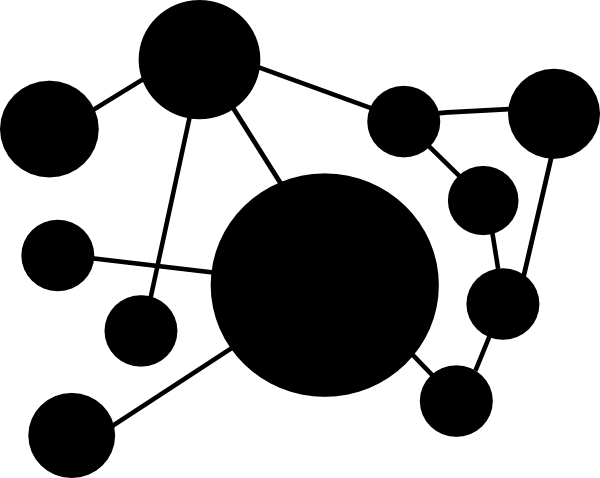
\includegraphics[width=50mm]{Bilder/Deckblatt/titelbild.png}\bigskip\bigskip} 

\publishers{
\includegraphics[width=100mm]{Bilder/Deckblatt/TH-Logo.jpg}}

%Erstellte Überschrift zür Überschrift machen
\maketitle

%Verzeichnisse einlesen
%Römische Nummerierung % Protusion setzen
\pagenumbering{Roman}
\microtypesetup{protrusion=false}

%Verzeichnisse
\tableofcontents
\listoffigures
\listoftables
\listofformels
 
\clearpage
\microtypesetup{protrusion=true} 
\pagenumbering{arabic} 

%Der eigentliche Text beginnt hier

%Einleitung einlesen
\chapter{Einleitung}
\label{chapter:Einleitung}

\section{Motivation}
\label{section:Motivation}

Die Untersuchung und Extrapolation von Zeitreihen ist ein bedeutendes Thema in zahlreichen Gebieten. Typische Anwendungsbereiche sind zum Beispiel die Prognose von Wetterdaten, von Therapieverläufen in der  Medizin, von Arbeitslosenzahlen auf dem Arbeitsmarkt sowie von Börsenkursen. Um eine Zeitreihe möglichst genau zu extrapolieren, wird auf mehrere Hilfsmittel zurückgegriffen. Eins dieser Hilfsmittel können KNN (künstliche neuronale Netze)sein. 

Bei KNN handelt es sich um Netzwerke mit künstlichen Neuronen als Knoten, die mittels gerichteter Verbindungen Eingaben einlesen, weiterverarbeiten und die daraus resultierenden Ergebnisse an weitere Neuronen weiterleiten oder als Ergebnis ausgeben. Bei der Terminologie von KNN wird bewusst auf Begriffe der Biologie zurückgegriffen, da KNN das biologische Gehirn als Vorbild nutzen und dessen Herangehensweise auf analoger Weise umzusetzen zu versuchen. Man nennt das Verfahren dieser Netze aus diesem Grunde auch \textit{naturanaloge Verfahren}.

Warum sind diese Netze nun so interessant für Prognosen? Das Erstellen von zum Beispiel Börsenprognosen basiert in der Regel auf Auswertungen von Informationen verschiedener Quellen. Die Art von Auswertungen, wie Börsenexperten sie vornehmen, ist weder vollständig formalisierbar noch besonders exakt, da uneinheitlich und in weiten Zügen intuitiv. Besonders schwer ist hier das Ermitteln von \textit{nichtlinearen Zusammenhängen}. Ein KNN ist jedoch in der Lage, diese Zusammenhänge zu finden  und diese objektiv und vorurteilsfrei zu bewerten. Somit sind diese prinzipiell in der Lage, jedes beliebige Muster in jedem beliebigen Markt zu erkennen - auch solche, die noch nie zuvor von irgend jemand entdeckt wurden.

Ob und wie gut KNN zur Prognose geeignet sind, ist pauschal nicht zu beantworten. In manchen Gebieten mag die Prognosefähigkeit durchaus ausreichen. Je höher die geforderte Genauigkeit jedoch wird, desto diskutabler wird ein Einsatz von KNN. Eine typische Grauzone ist hier wieder die Prognose von Börsenkursen. Während Befürworter auf die Eigenschaft von KNN hinweisen, nichtlineare Muster zu erkennen und entsprechend zu behandeln, argumentieren Kritiker, dass ein System, das dem menschlichen Lernen nachempfunden wurde, die gleichen Fehler machen wird wie der Mensch. Generell ist jedoch zu sagen, dass die Prognosequalität von KNN über die Jahre stets angestiegen ist, da zum einen stets neue Fortschritte in diesem Themengebiet gemacht werden und zum anderen die Leistungsfähigkeit von Rechners stetig ansteigt. 

\section{Ziel der Arbeit}
\label{section:Ziel der Arbeit}
In dieser Seminararbeit sollen KNN erschaffen werden, die in der Lage sind, Börsenkurse zu prognostizieren. Konkret sollen drei verschiedene KNN konzeptioniert und umgesetzt werden. Ein KNN zur Prognose des Kurses vom DAX (Deutschen Aktienindx), eines zur Prognose des Kurses vom Nikkei sowie eines zur Prognose des Kurses vom Dow Jones. Diese KNN sollen anschließend in einer Webanwendung überführt werden. Diese soll die Prognosefähigkeit der KNN visualisieren und Vergleiche zwischen einzelne Prognosen ermöglichen. In dieser Seminararbeit liegt der Fokus auf das Erlangen eines Grundverständnisses über KNN und nicht auf das komplette Ausreizen der Prognosefähigkeit von KNN. Trotzdem spielt die Prognosequalität der erstellten KNN eine wichtige Rolle in dieser Seminararbeit.

%Konzepton einlesen
\chapter{Konzeption}
\label{chapter:Konzeption}

\section{Konzeption der Anwendung} %Benedikt
\label{section:Konzeption der Anwendung} %Benedikt
<<Benedikt>>

\subsection{Grundidee} %Benedikt
\label{subsection:Grundidee} %Benedikt
<<Benedikt>>

\subsection{Mockup} %Benedikt
\label{subsection:Mockup} %Benedikt
<<Benedikt>>

\section{Konzeption des künstlichen neuronalen Netzes}
\label{section:Konzeption des künstlichen neuronalen Netzes}

In den folgenden Abschnitten wird ein \acs{knn} konzeptioniert, dass als Vorlage für alle zu erstellenden \acs{knn} zur Prognose von Börsenkursen dienen soll. 

\subsection{Wahl des Netztyps}
\label{subsection:Wahl des Netztyps}
Zunächst ist zu ermitteln, welche Netztypen sich zur Prognose von Börsenkursen grundsätzlich eignen. Nicht jeder Netztyp ist gleichermaßen zur Prognose geeignet. Bestimmte \acs{knn} sind beispielsweise überhaupt nicht in der Lage, Prognosen zu erstellen. 

Grundsätzlich lassen sich \acs{knn} in zwei Oberklassen unterteilen. Es gibt hetero-assoziative Netze sowie die auto-assoziative Netze. Hetero-assoziative Netze bilden einen Vektor $A$ der Länge $n$ auf einem Vektor $B$ einer meist kürzeren Länge $m$ $\{m \in \mathbb{N} | m \le n\}$ ab. Auto-assoziative Netze wiederum bilden einen Eingabevektor der Länge $n$ auf einem Ausgabevektor der gleichen Länge ab. Innerhalb dieser zwei Klassen lassen sich \acs{knn} wiederum in mehrere Netztypen aufteilen. Die folgende Tabelle liefert hierzu eine Übersicht:

\begin{center}
\begin{tabular}{|c|c|}
\hline 
\textbf{Hetero-assoziative Netzmodelle} & \textbf{Auto-assoziative Netzmodelle} \\ 
\hline 
(M)Adaline & Hopfield-Netze \\ 
\hline  
Perzeptron &  Boltzmann Maschinen \\ 
\hline 
Multilayerperzeptron & - \\ 
\hline 
\end{tabular} 
\end{center}

Das \acs{knn} soll mithilfe von mehreren vorhergehenden Börsenkursen den zukünftigen Börsenkurs prognostizieren. Da es sich bei den zu prognostizierenden Börsenkurs um einen skalaren Wert handelt, ist die Anzahl der Eingabeneuronen (und damit die Anzahl der Elemente des Eingabevektors) höher als die Anzahl der Ausgabeneuronen (und damit höher als die Anzahl der Elemente des Ausgabevektors). Somit sind für diese Seminararbeit nur hetero-assoziative Netze von Relevanz.

Aus der Menge der hetero-assoziativen Netze ist nun der Netztyp zu ermitteln, der für die Anwendung am geeignetsten ist.

Zur Wahl eines geeigneten Netztyps kann zunächst die Lineare Separierbarkeit betrachtet werden:

\newmdtheoremenv{defi}{Definition}
\begin{defi}Definition der linearen Separierbarkeit\\
Seien $X_{0}$ and $X_{1}$ zwei Datenmengen im $n$-dimensionalen euklidischen Raum. Dann sind die Mengen $X_{0}$ and $X_{1}$ genau dann  "`linear separierbar"', wenn es  $n+1$ Werte $w_{1}, w_{2},..,w_{n}, k$, gibt, sodass jeder Punkt  $x \in X_{0}$ die Bedingung $\sum^{n}_{i=1} w_{i}x_{i} > k$ erfüllt und jeder Punkt $x \in X_{1}$ die Bedingung $\sum^{n}_{i=1} w_{i}x_{i} < k$ erfüllt.
\end{defi}

Um das Verständnis der oben genannten Definition zu erleichtern, kann die folgende Abbildung betrachtet werden:

\begin{figure}[H]
\centering
		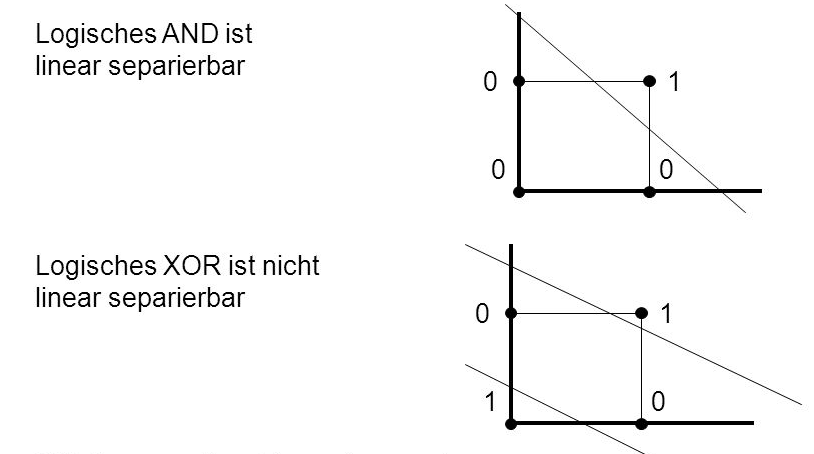
\includegraphics[width=0.95\textwidth]{Linear_Sep.PNG}
	\caption{Bildliche Erläuterung der linearen Separierbarkeit}
	\label{fig:Bildliche Erläuterung der linearen Separierbarkeit}
\end{figure}

Man erkennt also, das eine zweidimensionale Funktion dann als linear separierbar gilt, wenn zwischen zwei Ergebnismengen der Funktion eine Gerade gelegt werden kann. Analog setzt sich dies in Funktionen höherer Dimensionen fort. Ist die Funktion zum Beispiel dreidimensional, erfolgt die Separierung durch eine Ebene.

Es ist bewiesen, dass einschichtige \acs{knn} nur in der Lage sind, linear separierbare Funktionen zu berechnen. Den Konkreten Beweis dazu liefern Minski \& Papert am Beispiel des XOR-Problems:

\newmdtheoremenv{bew}{Beweis}
\begin{bew}Beweis der Eingeschränkten Fähigkeit von KNN anhand des XOR-Problems\\

Gegeben sind:\\

Ein Perzetron der folgenden Bauart:

\begin{figure}[H]
\centering
		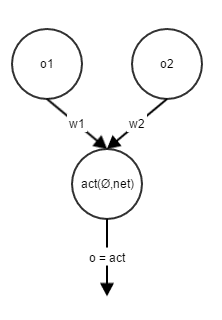
\includegraphics[width=0.20\textwidth]{Perzeptron.PNG}
	\caption{Beispielperzeptron zur Darstellung des XOR-Problems}
	\label{fig:Beispielperzeptron zur Darstellung des XOR-Problems}
\end{figure}

und folgende Rahmenbedingungen:

$w_1\cdot1 + w_2\cdot2 = net$\\ 
$f_(act)(o) = id$ \\
$\emptyset = Schwellenwert$

Dann gilt folgendes:\\
$a) w_1\cdot0 + w_2\cdot0 \le \emptyset$ Bei einem Inputvektor (0,0) liefert der Output 0.\\
$b) w_1\cdot0 + w_2\cdot0 \geq \emptyset$ Bei einem Inputvektor (0,1) liefert der Output 1.\\
$c) w_1\cdot0 + w_2\cdot0 \geq \emptyset$ Bei einem Inputvektor (1,0) liefert der Output 1.\\
$d) w_1\cdot0 + w_2\cdot0 \le \emptyset$ Bei einem Inputvektor (1,1) liefert der Output 0.\\

Der Widerspruch ergibt sich wie folgt:\\ $(b+c):  w_1 + w_2 \geq \emptyset  \wedge (d)  w_1 + w_2 \leq \emptyset$
\end{bew}

Dieser Beweis kann ebenfalls auf andere nicht linear separierbare Funktionen angewandt werden.Somit steht fest, dass ein einschichtiges Perzeptron nicht in der Lage sein kann, nicht linear separierbare Funktionen zu approximieren.

Auf Basis der oben genannten Tatsache kann ermittelt werden, ob ein einschichtiges Perzeptron zur Approximation von Börsenkursen geeignet ist. Dafür wurde ein ein Perzeptron folgender Bauart entwickelt und untersucht, ob dieses Konvergiert.

\begin{figure}[H]
\centering
		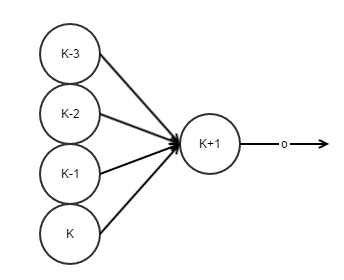
\includegraphics[width=0.5\textwidth]{Testperzeptron.PNG}
	\caption{Grundlegendes Konzept des KNN}
	\label{fig:Grundlegendes Konzept des KNN}
\end{figure}

Bei Betrachtung des Netzwerkfehlers des Perzeptrons erkennt man, dass das Perzeptron nicht konvergiert:

\begin{figure}[H]
\centering
		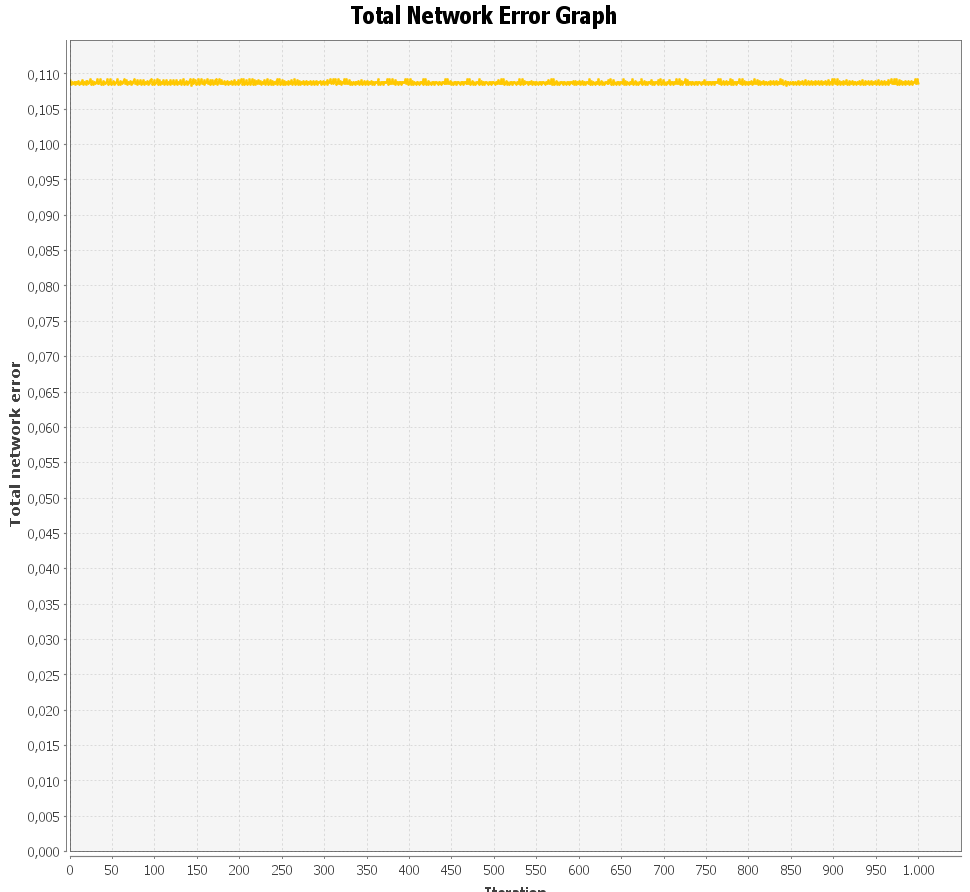
\includegraphics[width=0.5\textwidth]{MSEperzeptron.PNG}
	\caption{Grundlegendes Konzept des KNN}
	\label{fig:Grundlegendes Konzept des KNN}
\end{figure}

Der Netzwerkfehler des Perzeptrons bleibt über alle Iterationen konstant auf einen Niveau von circa $0,10$.

Nun ist es sinnvoll, folgendes Theorem zu berücksichtigen:
 
\newmdtheoremenv{theo}{Theorem}
\begin{theo}Konvergentheorem von Rosenblatt\\
Der Lernalgorithmus des Perzeptrons konvergiert in endlicher Zeit, d.h. das Perzeptron kann in endlicher Zeit alles lernen, was es repräsentieren kann.
\end{theo}

Betrachtet man alle oben genannten mathematischen Gegebenheiten, ergibt sich die folgende Relation:

Perzeptron konvergiert $\rightarrow$ Funktion Linear separierbar $\rightarrow$ Perzeptron geeignet.
und natürlich analog:Perzeptron konvergiert nicht $\rightarrow$ Funktion nicht Linear separierbar $\rightarrow$ Perzeptron nicht geeignet.

Folglich bleibt nur noch das Multilayerperzeptron als Mögliche Auswahl übrig. Das dieses \ac{knn} tatsächlich zur Prognose geeignet ist, belegt das folgende Theorem:

\begin{theo}Theorem von Kolmogorov\\
Für ${n \in \mathbb{N} | n>2}$ lässt sich jede reellwertige Funktion $f:[0;1]^n\rightarrow[0;1]$ durch ein dreischichtiges vorwärtsverknüpftes Netz mit maximal $n$ Einheiten in der Eingabeschicht,$(2n+1)$ Einheiten in der Zwischenschicht und $2n+1$ Einheiten in der Ausgabeschicht berechnen.
\end{theo}

Ein Börsenkurs kann prinzipiell jede beliebige Funktion annehmen. Durch das obige Theorem ist jedoch sichergestellt, dass das mehrschichtige vorwärtsgerichtete Netz in der Lage ist, diese Funktionen zu approximieren, da ein Multilayerperzeptron als universeller Aprroximator fungiert.

\subsection{Wahl der Topologie}
\label{subsection:Wahl der Topologie}

Zur Prognose des Börsenkurses sollen die letzten vier Börsenkurse als Input dienen. Durch diesen Input soll der Börsenkurs am nächsten Tag prognostiziert werden. Zur richtigen Dimensionierung der inneren Schicht können einige Richtlinien berücksichtigt werden:

\begin{itemize}
\item Die Anzahl der versteckten Neuronen in der inneren Schicht sollte nicht zu groß gewählt werden, damit das Netz das antrainierte Verhalten nicht "'auswending`" lernt und dieses dann nur bereits trainierte Muster anwenden kann und es somit die Generalisierungsfähigkeit verliert. Man spricht in diesem Fall von Overfittin.g 
\item Die Anzahl der versteckten Neuronen in der inneren Schicht sollte auch nicht zu klein gewählt werden, da eine gewisse Menge an Neuronen wichtig sind, um sich Regeln merken zu können.
\item Eine grobe Annäherung zur Bestimmung der Obergrenze der Anzahl von Neuronen in der versteckten Schicht liefert die folgende Formel:

\begin{equation}\formelentry{Optimale Anzahl Neuronen in der versteckten Schicht}
  N_h = \frac{N_d}{10*(N_i+N_o)}
\end{equation}
Nh ist hierbei die Obergranze, Ni ist die Anzahl der Inputneuronen und No die Anzahl der Outputneutonen. Da 450 Trainingsdaten verwendet werden. Bedeutet das für diese SEminararbeit konkret:

\begin{equation}\formelentry{Optimale Anzahl Neuronen in der versteckten Schicht}
  N_h = \frac{450}{10*(4+1) = 9 }   
\end{equation}
\end{itemize}
 

Somit ergibt sich insgesamt die folgende Topoologie:

\begin{figure}[H]
\centering
		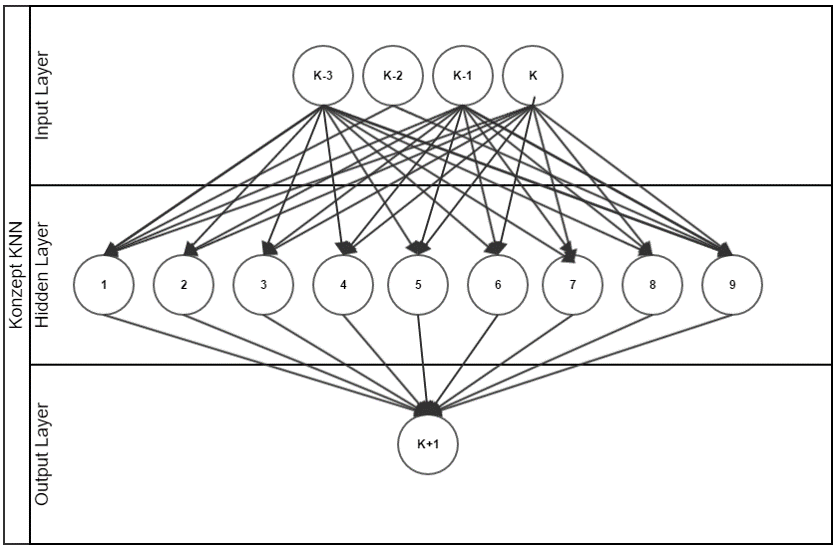
\includegraphics[width=0.5\textwidth]{KonzKNN.PNG}
	\caption{Grundlegendes Konzept des KNN}
	\label{fig:Grundlegendes Konzept des KNN}
\end{figure}


Die oben abgebildete Topologie stellt ein solides Grundkonstrukt dar, das in der Umsetzungsphase noch weiter optimiert werden kann.


\subsection{Wahl des Lernverfahrens} 
\label{subsection:Wahl des Lernverfahrens}

Grundsätzlich gibt es drei grobe Klassifikation von Lernverfahren. in diesem Abschnitt werden alle drei Lernverfahren näher vorgestellt und anschließend eine Begründete Auswahl der Lernverfahrens getroffen.

\begin{itemize}
\item Überwachtes Lernen
\item Bestärkendes Lernen
\item Unüberwachtes Lernen
\end{itemize}



%Umsetzung einlesen
\chapter{Umsetzung}
\label{chapter:Umsetzung}

In den folgenden Abschnitten wird auf die Umsetzung der Anwendung und des KNN eingegangen.

\section{Umsetzung der Anwendung}
\label{section:Umsetzung der Anwendung}
<<Benedikt>>\Blindtext

\section{Umsetzung des künstlichen neuronalen Netzes mit Neurophstudio} 
\label{section:Umsetzung des künstlichen neuronalen Netzes mit Neurophstudio}

In diesem Abschnitt wird beschrieben, wie das KNN aus der Konzeptionsphase (siehe Abbildung 2.3) umgesetzt wurde. Zur Umsetzung wurde die Anwendung "`Neurophstudio"' verwendet. Diese ist ein Teil des Neuroph-Frameworks und erlaubt das Erstellen, Trainieren und Testen von KNN mittels einer graphischen Oberfläche. Das erstellte KNN kann anschließend mittels einer Library in einer Java-Anwendung eingebunden werden.

Nachdem das grundlegende KNN in der Anwendung angelegt wurde, musste dieses noch trainiert und anschließend getestet werden. Für diesen Vorgang sind Trainings- sowie Testdaten nötig. Die benötigten Daten konnten als Excel-Datei von der nachfolgenden Webseite bezogen werden: \textit{http://www.quandl.com}. Es wurden die letzten $600$ Börsenkurse des DAX extrahiert und anschließend in $2$ Datensätze aufgeteilt: In einem Trainingsdatensatz bestehend aus $450$ Trainingsdaten sowie in einem Testdatensatz bestehend aus $150$ Testdaten. Da diese Datensätze noch nicht normalisiert waren, die Daten jedoch in normalisierter Form für das KNN zur Verfügung stehen müssen, wurden diese mit der folgenden Formel normalisiert:

\begin{equation}\formelentry{Normalisierungsformel}
  N_h = \frac{A)-min(A}{max(A)-min(A)}\cdot0,8+01
\end{equation}

Wobei $A$ den Datensatz als Matrix repräsentiert.

Damit wurde sichergestellt, dass sich alle Werte der Datensätze im Intervall $[0,1]$ befinden. Die Multiplikation mit $0,8$ sowie die Addition mit $0,1$ soll Extremwerte abmildern.

Nachdem alle Komponenten für die Erstellung eines fertigen KNN vorhanden waren, konnte mit dem Training begonnen werden. Dafür wurden $200.000$ Trainingszyklen gestartet. Als Lernverfahren wurde das Backpropagation-Verfahren mit einer Lernrate von $0,7$ benutzt und als Aktivierungsfunktion eine Sigmoide Funktion. Nachdem das Training abgeschlossen war, wurde das KNN noch entsprechend mit dem Testdatensatz getestet. Dabei haben sich jeweils die folgenden Werte ergeben:

\begin{table}[H]
\centering
\begin{tabular}{|c|c|}
\hline 
\textbf{Durchlauf} & \textbf{MSE} \\ 
\hline 
Trainingszyklus & 0,001048 \\ 
\hline  
Testzyklus & 0,002134  \\ 
\hline 
\end{tabular} 
\label{tab:ERGGrundnetz}
\caption{Die Trainings- und Testergebnisse des Grundnetzes}
\end{table}

Dieses KNN bildet nun die Grundlage für weitere Optimierungsmaßnahmen.

\section{Optimierung des künstlichen neuronalen Netzes}
\label{section:Optimierung des künstlischen neuronalen Netzes}

Nachdem das Grundmodell des KNN erstellt wurde, ist dieses noch weiter optimiert worden. Darauf wird nun in den Unterabschnitten \ref{subsection:Optimierung der Topologie}, \ref{subsection:Wahl der optimalen Transferfunktion} sowie \ref{subsection:Wahl der optimalen Lernregel} genauer eingegangen. 

\subsection{Optimierung der Topologie}
\label{subsection:Optimierung der Topologie}

Das im Abschnitt \ref{section:Umsetzung des künstlichen neuronalen Netzes mit Neurophstudio} erstellte KNN wird in diesem Abschnitt hinsichtlich der verwendeten Topologie optimiert. Dabei werden sukzessive Neuronen in der Zwischenschicht hinzugefügt bzw. entfernt und für jeden Trainings- und Testverlauf der MSE (Mean Squared Error) notiert. Auch wird jede Topologie einmal mit und einmal ohne ein Bias-Neuron trainiert und getestet. Die Topologie mit dem geringsten MSE im Testverlauf wird dann übernommen. Die Ergebnisse dieser Optimierung können aus der Tabelle \ref{tab:TOPMSE} entnommen werden. Der Buchstabe (B) steht dabei für das Bias-Neuron.

\begin{table}[H]
  \centering
  \begin{tabular}{|c|c|c|c|c|}
  \hline 
  \rule[0ex]{0pt}{2.5ex} \textbf{Topologie}& \textbf{Training-MSE} & \textbf{Test-MSE} & \textbf{Training-MSE (B)} & \textbf{Test-MSE (B}\\ 
  \hline 
  \rule[0ex]{0pt}{2.5ex} 4-03-1 (B)& $0.0011562$& $0.002569$ & $9.449 \cdot^{-4}$ & $0.001788$\\ 
  \hline 
  \rule[0ex]{0pt}{2.5ex} 4-05-1 (B)& $0.001062$ & $0.002879$ & $9.598 \cdot^{-4}$ & $0.001799$\\ 
  \hline 
  \rule[0ex]{0pt}{2.5ex} \textbf{4-07-1 (B)}& $0.001090$ & $0.001784$ & $9.407\cdot^{-4}$ & $0.001781$\\ 
  \hline 
  \rule[0ex]{0pt}{2.5ex} 4-09-1 (B)& $0.001048$ & $0.002134$ & $9.488\cdot^{-4}$ & $0.0024436$\\ 
  \hline 
  \rule[0ex]{0pt}{2.5ex} 4-11-1 (B)& $0.001022$ & $0.001785$ & $9.760\cdot^{-4}$ & $0.0033215$\\ 
  \hline 
  \rule[0ex]{0pt}{2.5ex} 4-13-1 (B)& $0.001002$ & $0.001787$ & $9.906\cdot^{-4}$ & $0.004067$\\ 
  \hline 
  \end{tabular} 
  \caption{Jeweilige Topologien \& korrespondierende MSE}
  \label{tab:TOPMSE}
\end{table}

Wie aus der Tabelle \ref{tab:TOPMSE} zu erkennen, liefert eine Topologie mit $4$ Input-Neuronen, $7$ versteckten Neuronen, ein Bias-Neuron sowie ein Output-Neuron die besten Testergebnisse. Die Start-Topologie aus der primären Umsetzung wird nun durch diese Topologie ausgetauscht.

\subsection{Wahl der optimalen Transferfunktion} 
\label{subsection:Wahl der optimalen Transferfunktion} 

Nachdem die Topologie des KNN optimiert wurde, ist noch die Transferfunktion optimiert worden. Hierbei wurde das Netz einmal mittels einer sigmoiden Funktion und anschließend nochmals mit der Tanh-Funktion trainiert und getestet. Dabei ist anzumerken, dass die Tanh-Funktion lediglich einen Sonderfall einer sigmoiden Funktion darstellt (Das wird klarer, wenn man bedenkt, dass "`Sigmoid"' mit "`S-Förmig"' übersetzt werden kann). Die Abbildung \ref{fig:sigtanh}
zeigt nochmals die Bauart der beiden Funktionen auf.

\begin{figure}[H]
\hfill
\subfigure[Sigmoid]{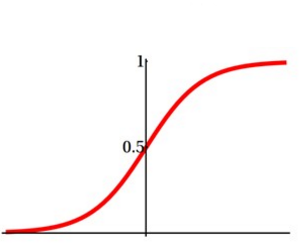
\includegraphics[width=5cm]{Sigmoid.PNG}}
\hfill
\subfigure[Tanh]{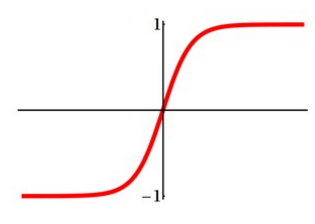
\includegraphics[width=5cm]{tanh.PNG}}
\hfill
\caption{Die Sigmoide Funktion und die Tanh Funktion im Vergleich}
\label{fig:sigtanh}
\end{figure}

\begin{equation}\formelentry{Sigmoide Funktion sowie Tanh Funktion}
(a)\ f(x)= \frac{1}{1+e^{-cx}}\ \ \ \ \ \ \ \ \ \ \ (b)\ f(x)= tanh(x)
\end{equation}


Aus der Tabelle \ref{tab:TRANSMSE} können die Ergebnisse dieses Optimierungsschrittes entnommen werden.


\begin{table}[H]
  \centering
  \begin{tabular}{|c|c|c|}
  \hline 
  \rule[0ex]{0pt}{2.5ex} Transferfunktion & Training-MSE & Test-MSE \\ 
  \hline 
  \rule[0ex]{0pt}{2.5ex} \textbf{Sigmoid} & $9.406 \cdot 10^{-4}$ & $0.001767$\\ 
  \hline 
  \rule[0ex]{0pt}{2.5ex} Tanh & $0.0103333$ & $0.044330$ \\ 
  \hline 
  \end{tabular} 
  \caption{Jeweilige Transferfunktionen \& korrespondierende MSE}
  \label{tab:TRANSMSE}
\end{table}

Man erkennt, dass es sich bei der bisher genutzten sigmoiden Funktion bereits um die beste Lösung handelt. Folglich wurde das KNN in dieser Hinsicht nicht weiter optimiert und die ursprüngliche Funktion wurde belassen.

\subsection{Wahl der optimalen Lernregel}
\label{subsection:Wahl der optimalen Lernregel}

Als letzten Schritt wurde die Lernregel des KNN optimiert. Innerhalb des Verfahrens der überwachten Lernens existieren mehrere Lernregeln, um das Netz zu trainieren. Die bekannteste Lernregel ist die Backpropagation-Lernregel. Diese Regel gibt es in mehreren Variationen. In dieser Seminararbeit werden zum einen das Grundverfahren sowie einige Variationen, namentlich das  "`Momentum Backpropagation"' sowie das "`Resilient Backpropagation"' beschrieben und untersucht. Anschließend wird das für die Anwendung am besten geeignete Verfahren ausgewählt\footnote{\Vgl\Zitat{Laemmel}, S. 225 f.}.

\begin{itemize}
\item \textbf{Backpropagation}:\\
Dies ist das klassische Fehlerrückführungsverfahren zum Anpassen der Verbindungsgewichte. Die Gewichtsveränderung erfolgt durch ein Fehlersignal, dass aus der Abweichung von tatsächlicher und prognostizierter Ausgabe berechnet wird. Die Gewichtsveränderung erfolgt hierbei schichtweise von den Ausgangs-Neuronen bis zu den Eingangs-Neuronen.

\item \textbf{Momentum Backpropagation}:\\
Dieses Verfahren fügt dem klassischen Verfahren einen Trägheitsterm hinzu, indem die Gewichtsveränderung zum Zeitpunkt $t-1$ berücksichtigt wird. Dieser Term kann einen Wert zwischen $0$ und $1$ annehmen. Umso größer dieser Term ist, umso stärker wir die vorhergehende Gewichtsveränderung berücksichtigt. Durch diesen Trägheitsterm wird die Wahrscheinlichkeit verringert, dass das KNN beim Training in ein lokales Minimum oszilliert und sich somit nicht weiter dem Idealwert approximieren kann. Auch die Wahl der Lernrate gestaltet sich hier weniger kritisch. 

\item \textbf{Resilient Propagation}:\\
Resilient heißt Federnd. Dieses Verfahren nutzt das Vorzeichen das Gradienten zum Zeitpunkt $t$ und entscheidet anhand dessen, ob das Gewicht vergrößert oder verkleinert werden muss. Der Betrag der Gewichtsveränderung wird jedoch unabhängig von der Richtung der Gewichtsänderung ermittelt.  Dadurch werden die typischen Probleme klassischer Gradientenabstiegsverfahren, wie sie beim klassischen Backpropagation sowie beim Momentum Backpropagation genutzt werden, gemindert.\footnote{\Vgl\Zitat{Valen}, S. 71}.

Die Formeln für Resilient Propagation lauten wie folgt:

\begin{equation}\formelentry{Formel zur Bestimmung der Art der Gewichtsänderung}
\Delta w_{ij}=\begin{cases} 
-\Delta_{ij} & falls S(t) > 0 \\ 
+\Delta_{ij} & falls S(t) < 0  \\ 
\pm 0       & sonst 
\end{cases}
\end{equation}

\begin{equation}\formelentry{Formel zur Bestimmung des Betrages der Gewichtsänderung}
\Delta_{ij}=\begin{cases} 
\Delta_{ij}(t-1)\cdot n^+ & falls S(t-1) \cdot S(t) > 0 \\ 
\Delta_{ij}(t-1)\cdot n^- & falls S(t-1) \cdot S(t) < 0 \\
\Delta_{ij}(t-1)       & sonst 
\end{cases}
\end{equation}


Solange sich das Vorzeichen des Gradienten negativ ist, wird das Vorzeichen beibehalten und die Schrittweite und somit das Gewicht um einen konstanten Wert $n^{+}$ vergrößert. Somit können Plateaus besser überwunden werden.
Ändert sich das Vorzeichen des Gradienten von negativ auf positiv(was bedeutet, dass ein Minimum übersprungen wurde) so wird das Vorzeichen geändert und die Schrittweite um  einen fixen Faktor $n^{-}$ verringert. Somit werden Oszillationen verhindert.

Die Abbildung \ref{fig:RP} stellt das Vorgehen des Resilient Propagation Algorithmus grafisch dar\footnote{\Vgl\Zitat{Geith}, S. 71}.

\begin{figure}[H]
	\centering
	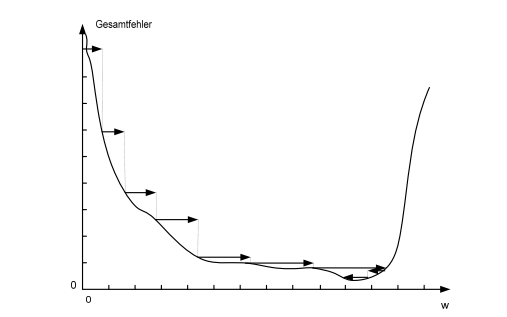
\includegraphics[width=10cm]{VisuResi.PNG}
	\caption{Visualisierung des Resilient Propagation Algorithmus}
	\label{fig:RP}
\end{figure}

\end{itemize}

Allen drei Lernregeln ist gemein, dass zur Bestimmung des Fehlers zwischen der prognostizierten und tatsächlichen Ausgabe der MSE benutzt werden kann. Die MSE-Formel würde in dem konkreten Fall der Anwendung wie folgt lauten:

\begin{equation}\formelentry{MSE zur Berechnung der Abweichung}
   \frac{1}{2}\sum^{n}_{i=1} (KT_{i} - KV_{i})^2
\end{equation}

Wobei $n$ für die Anzahl der Daten im Datensatz steht, $KT_i$ für den tatsächlichen Ausgabewert eines Datum $i$ steht und $KV_i$ für den korrespondierenden prognostizierten Ausgabewert eines Datums $i$ steht.

In der Tabelle \ref{tab:LERNregeln} kann das Ergebnis der Trainings- und Testdurchläufe mit den jeweiligen Lernregeln betrachtet werden.

\begin{table}[H]
  \centering
  \begin{tabular}{|c|c|c|}
  \hline 
  \rule[0ex]{0pt}{2.5ex} Lernregel & Training-MSE & Test-MSE \\ 
  \hline 
  \rule[0ex]{0pt}{2.5ex} Backpropagation & $9.325\cdot10^{-4}$ & $0.001636$ \\ 
  \hline 
  \rule[0ex]{0pt}{2.5ex} Momentum Backpropagation & $9.109\cdot10^{-4}$ & $0.001608$ \\ 
  \hline 
  \rule[0ex]{0pt}{2.5ex} \textbf{Resilient Propagation} & $8.89\cdot10^{-4}$ & $9.406\cdot10^{-4}$ \\ 
  \hline 
  \end{tabular} 
  \caption{Lernregeln \& jeweilige MSE}
  \label{tab:LERNregeln}
\end{table}

In der Regel liefert Resilient Propagation sehr gute Ergebnisse, dies ist auch hier der Fall. Wie man erkennen kann, ist das Resilient Propagation Verfahren  hier den anderen überlegen. Folglich wurde das KNN entsprechend optimiert und Resilient Propagation als Lernregel eingesetzt. Da es sich bei Resilient Propagation um eine adaptive Lernregel handelt und bei der Berechnung keine Lernrate benutzt handelt, muss diese auch nicht angegeben werden.

\section{Die endgültigen künstlichen neuronalen Netze}
\label{section:Die endgültigen künstlichen neuronalen Netze}

Nachdem das KNN zur Prognose des DAX erstellt und optimiert wurde, wurden diese Schritte in analoger weise für die KNN zur Prognose des Nikkei sowie zur Prognose des Dow Jones wiederholt.
Es stellte sich heraus, dass das optimale KNN für den DAX ebenfalls das Optimale KNN für den Nikkei und den Dow Jones darstellt. Das Endgültige Netz sowie dessen Parameter können aus der Tabelle \ref{tab:ENDconf} sowie aus der  Abbildung \ref{fig:ENDKNN} entnommen werden.

\begin{table}[H]
  \centering
  \begin{tabular}{|c|c|}
  \hline 
  \rule[0ex]{0pt}{2.5ex}  Topologie & 4-7-1 mit Bias\\ 
  \hline 
  \rule[0ex]{0pt}{2.5ex}  Lernregel & Resilient Propagation\\  
  \hline 
  \end{tabular} 
  \caption{Die jeweiligen Börsenkurse \& deren Endwerte}
  \label{tab:ENDconf}
\end{table}

\begin{figure}[H]
	\centering
	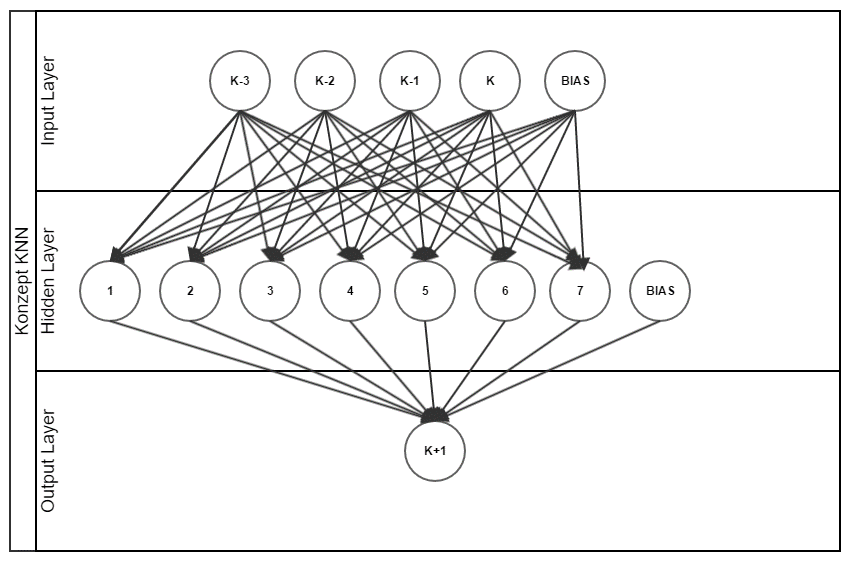
\includegraphics[width=10cm]{FertigKNN.PNG}
	\caption{Das endgültige KNN für alle Börsenkurse}
	\label{fig:ENDKNN}
\end{figure}

Die Tabelle \ref{tab:ENDval} zeigt die Trainings- sowie Testergebnisse der implementierten und optimierten KNN nach jeweils $200.000$ Trainingszyklen.

\begin{table}[H]
  \centering
  \begin{tabular}{|c|c|c|}
  \hline 
  \rule[0ex]{0pt}{2.5ex}  Börsenkurs & Training-MSE & Test-MSE\\ 
  \hline 
  \rule[0ex]{0pt}{2.5ex} DAX & $4.252\cdot10^{-5}$ & $4.820\cdot10^{-5}$  \\ 
  \hline 
  \rule[0ex]{0pt}{2.5ex} Nikkei & $1.350\cdot10^{-5}$ & $4.520\cdot10^{-5}$  \\ 
  \hline 
   \rule[0ex]{0pt}{2.5ex} Dow Jones & $6.672\cdot10^{-5}$ & $2.820\cdot10^{-4}$  \\ 
  \hline 
  \end{tabular} 
  \caption{Die endgültigen Parameter für alle KNN}
  \label{tab:ENDval}
\end{table}

\section{Zusammenführung der Komponenten}
\label{section:Zusammenführung der Komponenten}
<<Benedikt>> \Blindtext


%Beschreibung der Anwendung einlesen
\chapter{Beschreibung der Anwendung} %Benedikt
\section{Elemente der GUI} %Beide
\section{Architektur der Anwendung} %Benedikt

%Analyse der Anwendung einlesen
\chapter{Analyse}
\Blindtext

%Fazit einlesen
\chapter{Fazit} %Beide
\label{cha:Fazit}
\Blindtext

%Literaturverzeichnis anzeigen
\bibliographystyle{plain}
\bibliography{Literatur}

\end{document}
%%Body------------------------------------------------------